% !TEX root = ../main.tex
\chapter{Introduzione}
Nel progetto sono stati affrontati alcuni dei vari problemi che riguardano l'intelligenza artificiale. In questa relazione spiegheremo quali soluzioni sono state adottate, i vantaggi e gli svantaggi e alcuni miglioramenti che possono esser fatti al nostro progetto.

\section{Strategie}
Per svolgere il progetto di IA-LAB sono state implementate 4 strategie in maniera incrementale:
\begin{itemize}
  \item FIFO WAIT: la strategia usa la politica fifo come politica di scelta degli ordini.
  \item FIFO PRO: Simile alla precendente, ma in caso di ostacolo che non permette di servire un ordine, l'ordine viene messo al fondo.
  \item LOW PENALITY: strategia che si basa sulla penalità per effettuare la scelta dell'ordine.
  \item HARD: a differenza delle altre 3 strategie, questa permette di gestire più ordini in contemporanea. Come la precedente si basa sulle penalità.
\end{itemize}

Ogni strategia è stata suddivisa in fasi dove ogni fase si occupa di uno specifico sotto-problema. Questa suddivisione ci ha permesso sia uno sviluppo incrementale all'interno della stessa strategia, sia tra strategie diverse, dove è bastato andare a sviluppare in modo più articolato una fase oppure nell'inserire nuove fasi.

Nelle prime due strategie utilizzeremo come astrazione il concetto di coda. Gli ordini verranno inseriti in coda e prelevati dalla testa, quindi prelevati in ordine crescente di step.

\subsection{Il modulo A*}
\label{sec:modulo_astar}
Tutte le strategie utilizzano il modulo A* per la costruzione dei piani che permettono al nostro robot di spostarsi da un punto A a un punto B. Il punto A è la posizione del robot al momento della pianificazione mentre il goal (il punto B) è dato dalla cella destinazione. Il goal può essere un dispenser, un cestino o un tavolo. Il modulo A* calcolerà anche quali sono i 4 punti di accesso alla nostra destinazione e si fermerà non appena arriverà a uno di esso.

Il modulo A* può terminare fornendo un piano, oppure può fallire. Per memorizzare il piano creato vengono usate due strutture:

\begin{lstlisting}
(deftemplate plane
	(slot plane-id)
	(multislot pos-start)
	(multislot pos-end)
	(slot direction)
	(slot cost)
	(slot status (allowed-values ok failure))
)
\end{lstlisting}

\begin{lstlisting}
(deftemplate step-plane
	(slot plane-id)
	(slot action)
	(slot direction)
	(multislot pos-start)
	(slot father)
	(slot child)
)
\end{lstlisting}

La struttura step-plane indica i vari passi per eseguire il piano \emph{plane}. I piani vengono memorizzati in modo tale che il robot non debba ripianificare più volte uno stesso percorso. Vengono memorizzati solo i piani principali; nel caso in cui un piano fallisca il piano \emph{riparatore} non viene memorizzato.

\chapter{Strategie}
\section{Strategia FIFO WAIT}
La prima strategia che illuestreremo è la FIFO WAIT. \'E una strategia molto semplice, dove gli ordini vengono gestiti come una coda FIFO. Ci sono tre tipi di ordini, gestiti internamente alla strategia e sono diversi i modi in cui essi vengono completati:\begin{itemize}
  \item Ordine Accepted: un ordine di questo tipo verrà completato solo quando verranno consegnate al tavolo tutte le consumazioni richieste.
  \item Ordine Delayed: un ordine di questo tipo verrà completato solo quando verranno consegnate al tavolo tutte le consumazioni richieste. Rispetto al caso precedente le consumazioni non potranno esser consengate fin quando il tavolo non verrà pulito e le consumazioni buttate nel cestino.
  \item Ordine Finish: un ordine di questo tipo verrà completato solo quanto verrà pulito il tavolo e il robot butterà lo sporco nei vari cestini.
\end{itemize}
\newpage

\begin{figure}[htp]
  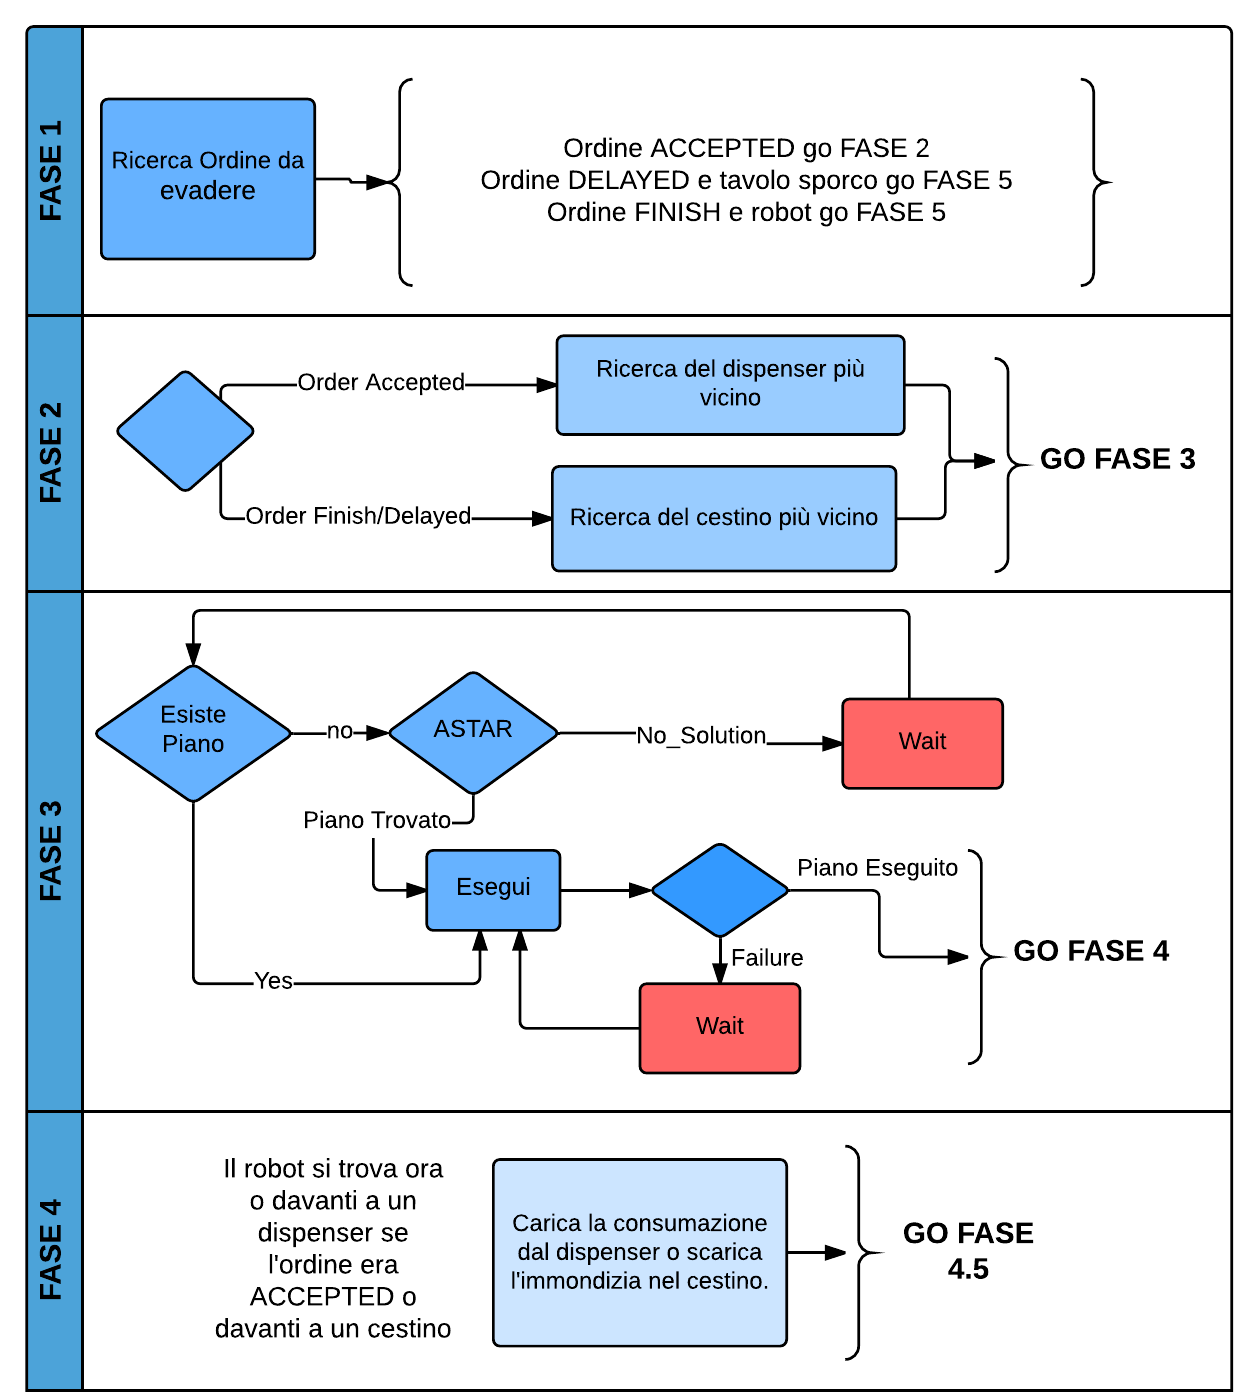
\includegraphics[width=\textwidth]{schema-fifo-wait1.png}
  \caption{Schema Fifo Wait}
  \label{fig:figure1}
\end{figure}

\begin{figure}[htp]
  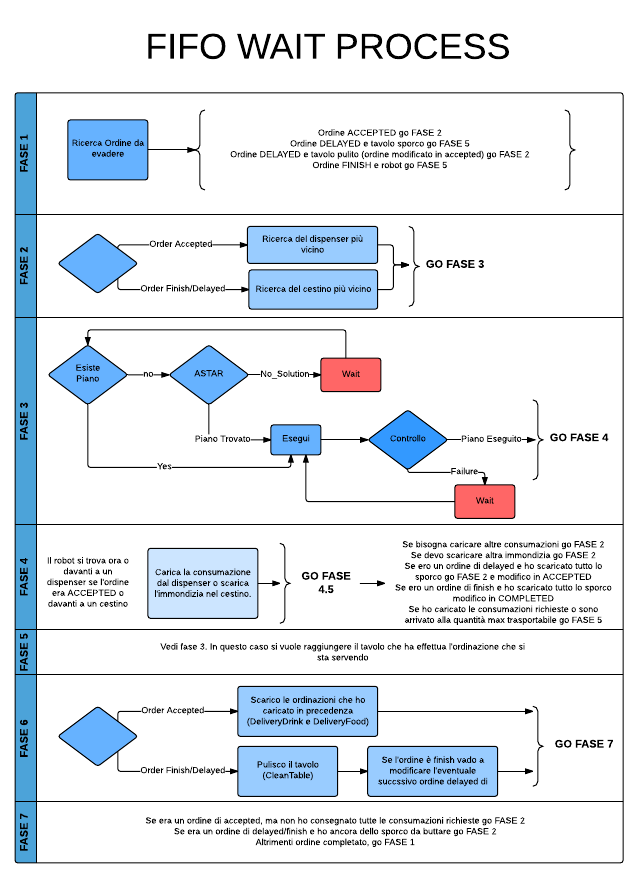
\includegraphics[width=\textwidth]{schema-fifo-wait2.png}
  \caption{Schema Fifo Wait}
  \label{fig:figure2}
\end{figure}

Come possiamo vedere dallo schema abbiamo suddiviso la nostre strategia in 7 fasi:
\begin{itemize}
  \item Fase 1: Nella prima fase viene individuato quale sarà l'ordine da servire. Ipotizzando di avere una coda in cui gli inserimenti vanno in coda e i prelievi avvengono dalla testa, l'ordine da evadere sarà l'ordine arrivato da più tempo cioè quello che ha un valore di step più basso.
  \item Fase 2: In questa fase si andrà ad individuare quale sarà il cestino o il dispenser presso il quale il nostro robot dovrà recarsi. La ricerca del cestino o del dispenser dipende dal tipo di ordine.
  \item Fase 3: In questa fase il robot arriverà alla destinazione prefissata. Per far ciò deve prima calcolare un piano con A* e poi eseguirlo. Il piano viene calcolato solo se non ne esiste già uno. In caso A* non trovi soluzione il robot esegue una wait e prova a ricalcolare A* fin quando non trova una soluzione.
  Quando il robot ha un piano per raggiungere la sua destinazione lo esegue. Nel caso in cui il piano fallisca il robot esegue una wait e prova a rieseguirlo.
  \item Fase 4: Il robot a seconda dell'ordine che sta servendo si troverà davanti un dispenser per caricare delle consumazioni (ordine \emph{accepted}) oppure davanti a un cestino per buttare lo sporco (ordine \emph{delayed} o \emph{finish}).
  \item Fase 4.5: Questa è la fase di controllo in cui il robot decide cosa deve fare, a seconda dell'ordine attivo. Per esempio se era un ordine accepted e ha caricato solo i \emph{food} e gli mancano i \emph{drink} dovrà ritornare alla fase 2; analogamente se era un ordine di finish o delayed e deve ancora buttare dello sporco.
  \item Fase 5: Identica alla fase 3 tranne per il fatto che la destinazione sarà un tavolo.
  \item Fase 6: Il robot in questa fase si trova in una posizione in cui può operare sul tavolo. Nel caso di ordine accepted rilascio tuttle le consumazioni caricate; in caso di ordine finish o delayed pulisco il tavolo.
  \item Fase 7: In questa fase controllo se l'ordine può essere considerato completato.
\end{itemize}

\subsection{Vantaggi e Svantaggi}
Vantaggio di questa strategia è sicuramente la semplicità e l'intuibilità con la quale il sistema funziona. L'idea di questa strategia, oltra alla politica di evasione degli ordini che può essere cambiata in qualsiasi momento andando solo a modificare la fase 1, è quella che il mondo è dinamico e lo è con una certa frequenza.

\begin{wrapfigure}{r}{0.33\textwidth}
    \centering
    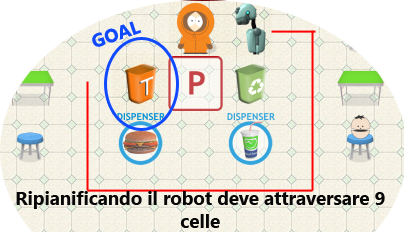
\includegraphics[width=0.33\textwidth]{Problema1_fifo_wait}
\end{wrapfigure}

L'assunzione dalla quale siamo partiti è che le persone si spostano e si spostano molto frequentemente. Da questo risulta evidente che se per arrivare in una determinata posizione incontro un ostacolo (una persona) la mossa più conveniente è quella di aspettare.
Se prendiamo in considerazione le teorie di Rodney Brooks in cui afferma che un comportamento intelligente è attribuibile da un osservatore esterno che vede l'agente interagire con l'ambiente, allora in alcune circostanze il nostro agente potrebbe non dimostrare tale comportamento intelligente. Se una persona rimane, anche se per pochi step in una posizione lungo il percorso dell'agente, il nostro agente invece di aggirarla e dimostrare un comportamento intelligente continuerà a provare a muoversi lungo la sua direzione fin quando la persona non si sarà spostata.

\begin{wrapfigure}{l}{0.25\textwidth}
    \centering
    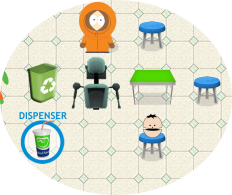
\includegraphics[width=0.25\textwidth]{Problema2_fifo_wait}
\end{wrapfigure}

Questo comportamento porta anche a situazioni di deadlock. Essendo in un ambiente simulato anche le persone non hanno un comportamento intelligente, supponendo che una persona si vuole spostare in direzione sud e il robot in direzione nord si arriva in una situazione di stallo. Per ovviare a questa problematica abbiamo implementato la strategia FIFO PRO.

\section{Strategia FIFO PRO}
La strategia FIFO PRO è un estensione della strategia FIFO WAIT per risolvere il "problema" riscontrato precedentemente. I concetti chiave che differenziano questa strategia dalla precendente sono 2:
\begin{itemize}
  \item ripianificazione nel caso un piano fallisca
  \item possibilità di cambiare l'ordine da servire se ci accorgiamo che non è possibile completarlo.
\end{itemize}

Il primo punto comporta delle modifiche nello schema visto in precedenza nella fase 3 e nella fase 5, ovvero nelle fasi delle ricerca ed esecuzione del piano. La figura \ref{fig:figure3} ci mostra le modifiche.

\begin{figure}[htp]
  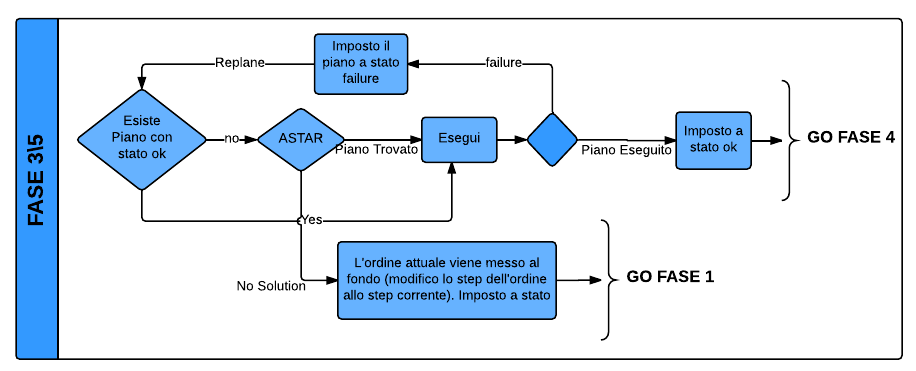
\includegraphics[width=\textwidth]{Fase3-FIFO-PRO}
  \caption{Fase 3 e 5 della strategia FIFO PRO}
  \label{fig:figure3}
\end{figure}

\newpage
\begin{wrapfigure}{r}{0.25\textwidth}
    \centering
    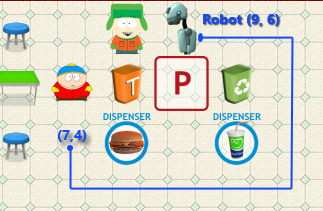
\includegraphics[width=0.25\textwidth]{Problema1_fifo_pro}
\end{wrapfigure}

Più complicate le conseguenze del secondo punto, che sono strettamente legate alla pianificazione. La pianificazione non trova sempre una soluzione. Nel caso in cui astar non riesca a trovare un percorso per raggiungere la nostra destinazione cambiamo l'ordine da servire. Questo comporta che l'ordine corrente verrà messo al fondo della nostra coda ordini e sarà servito successivamente. Questo commporta alcuni problemi che hanno complicato la stratgia FIFO PRO rispetto la precedente, e che saranno comuni anche alle successive strategie.

La strategia FIFO WAIT aveva un grosso vantaggio: ogni volta che si serve un nuovo ordine sicuramente l'agente si trova nello stato adatto per iniziare a servirlo.
Questo significa che l'agente non ha nè sporco nè consumazioni a bordo. Questa sicurezza non si ha nella strategia FIFO PRO. Supponiamo che un agente stia servendo un ordine finish e debba andare al cestino per liberarsi dallo sporco ma sfortunatamente il cestino non ha punti d'ingresso perchè occupati da persone, questo ordine verrà abbandonato e inserito al fondo e verrà recuperato il successivo ordine. Se il successivo ordine è un accepted non potrò subito avviare le operazioni per servirlo, ma dovrò sempre liberarmi dello sporco.

Nella fase 1 si ha un dispatcher che indica, a seconda dello stato dell'agente e dell'ordine, l'azione da compiere. La figura \ref{fig:figure4} mostra la fase 1 della strategia FIFO PRO.

\begin{figure}[htp]
  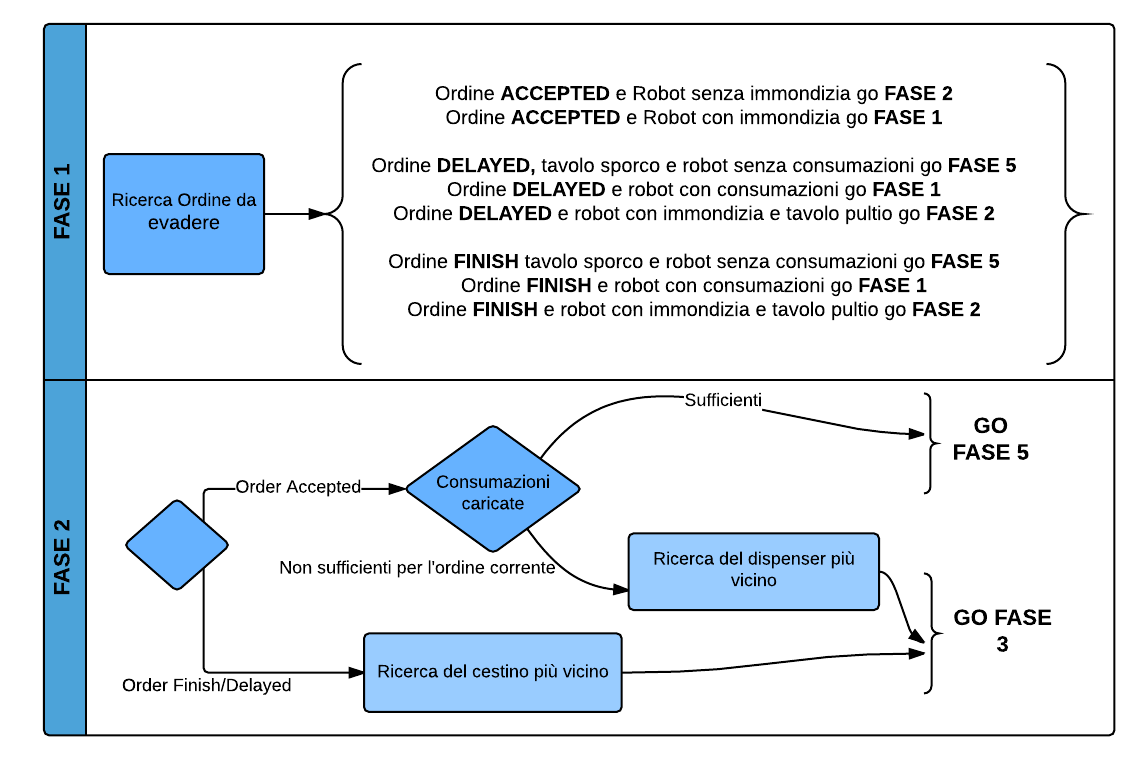
\includegraphics[width=\textwidth]{FIFO_PRO_fase1-2}
  \caption{Fase 1 e 2 della strategia FIFO PRO}
  \label{fig:figure4}
\end{figure}

Rimescolando gli ordini può succedere che ordini accepted vengano completati in ordine diverso dal quale siano arrivati. Nella stategia FIFO WAIT si era sicuri che una volta caricate le consumazioni dai dispenser, quelle consumazioni sarebbero state consegnata al tavolo che le aveva richieste. Nella strategia FIFO PRO questo non avviene. Supponendo di aver caricato dai dispenser un tot di consumazioni e che il robot non riesca ad arrivare al tavolo, il successivo ordine di accepted che verrà prelevato dalla coda potrebbe non aver bisogno di tornare ai dispenser (o di tornarci parzialmente), in quanto il robot ha già a bordo le consumazioni dell'ordine precedente. Si è dovuto implementare un meccanismo che permetta di capire al robot se e quanto deve caricare dai dispenser.

Altra piccola modifica avviene nella fase 6. Nella strategia FIFO WAIT gli ordini di tipo finish erano sicuramente eseguiti prima degli ordini di tipo delayed (questo comportava di andare a modificare l'ordine delayed in accepted una volta pulito il tavolo). Nella strategia FIFO PRO questo non è sempre vero, è possibile che un ordine finish venga rimesso al fondo della nostra coda e verrà eseguito un ordine di delayed (ovviamente ci riferiamo a ordini sullo stesso tavolo). In questo caso se l'ordine delayed riesce con successo a pulire il tavolo, il sistema dovrà settare come completata anche l'ordine finish.

Nella fase 7 inoltre quando il robot svuota l'immondizia bisogna andare a settare a completato tutti gli ordini finish che sono stati rimessi in coda perchè il dispenser era occupato.

\begin{figure}[htp]
  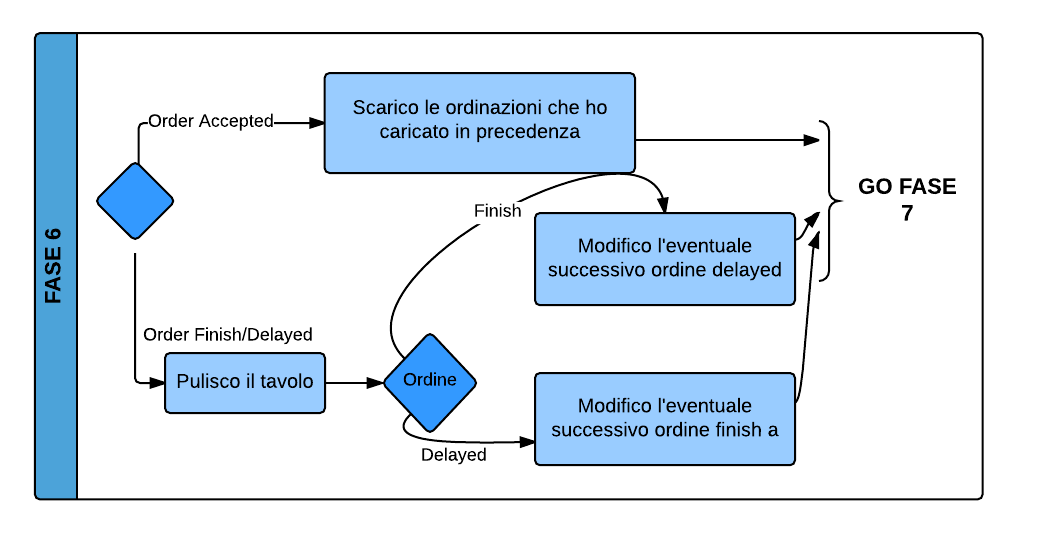
\includegraphics[width=\textwidth]{FIFO_PRO_fase6}
  \caption{Fase 6 della strategia FIFO PRO}
  \label{fig:figure5}
\end{figure}

\subsection{Vantaggi e Svantaggi}
Il sistema riesce dinamicamente a servire i vari ordini ripianificando i percorsi o cambiando gli ordini da servire. Obiettivo di questa strategia è rendere il sistema più robusto e flessibile.
Anche utilizzando questa strategia il sistema potrebbe rimanere bloccato, si veda la figura \ref{fig:figure6}. Si potrebbe ulteriormente ottimizzarla andando a imporre un numero di fallimenti massimo per arrivare a una specifica posizione; arrivati a tale limite l'ordine viene rimpiazzato dal successivo.


\begin{SCfigure}[]
\centering
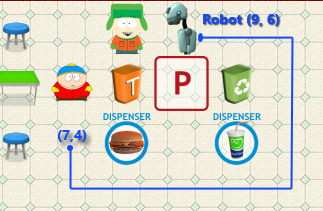
\includegraphics[width=0.40\textwidth]{Problema1_fifo_pro}
\caption{In questo esempio il robot vuole arrivare al TD e continuerà a spostarsi dalla cella (9,6) alla (7,4) e viceversa. Ricordiamo che il robot del mondo conosce solo lo stato delle 9 celle adiacenti a lui e le posizioni dei dispenser e dei tavoli. Quando si trova nella cella (7,4) non sa che nella (9,5) c'è una persona e quindi astar pianifica verso quella destinazione.}
\label{fig:figure6}
\end{SCfigure}

\section{Strategia LOW PENALITY}
\label{sec:lowpen}
La strategia LOW PENALITY si differenzia dalla precedente soprattutto per la Fase 1, ovvero per la ricerca dell'ordine da evadere. Si abbandona la politica FIFO per individuare e servire l'ordine che a ogni step porterebbe una penalità maggiore. Ogni qual volta arriva un ordine, viene calcolata la relativa penalità. Quando bisogna scegliere un ordine si sceglie quello con penalità maggiore. L' obiettivo è quello di minimizzare la penalità.
Altra differenza con le precedenti strategia sta nella gestione dell'ordine accepted. Nelle precedenti strategie l'ordine viene evaso completamente. In questa strategia si vuole minimizzare le penalità, quindi se un ordine ha richiesto 3 food e 3 drink, l'agente consegnerà le consumazioni secondo la sua massima capienza. Consegnate le consumazioni l'ordine o è stato completato o viene rimesso negli ordini da evadere aggiornando le consumazioni (e le penalità) in base a quelle già consegnate.

\subsection{Vantaggi e Svantaggi}
Obiettivo di questa strategia è quella di minimizzare le penalità rispetto alle strategia precedenti. Vedremo nella sezione Analisi Strategia se i risultati sono stati raggiunti. Gli svantaggi sono i medesimi della strategia FIFO PRO.

\section{Strategia PENDIST}
La strategia PENDIST (acronimo di PENality DISTance) usa come base di partenza la strategia precedente, la LOW PENALITY [vd. \ref{sec:lowpen}]; ne condivide dunque gli stessi pregi, in particolare il tentativo di servire l'ordine con penalità massima.

All'euristica che usiamo per cercare il tavolo da servire aggiungiamo un pezzo, ossia minimizzare la distanza in step in modo da completare l'ordine a massimo carico (la strategia low-penality, cerca di servire quel tavolo caricando il più possibile per quel singolo ordine, poi una volta completato la fase di portare il cibo&drink al tavolo e c'è ancora roba da servire, rimette il tavolo nel pool degli ordini da evadere e ricalcola la penalità.). Per minimizzare questo valore, utilizziamo il concetto di priorità, concetto che ci permette di scegliere l'obietivo con priorità più alta. La priorità di ogni obiettivo viene calcolata moltiplicando la sua penalità con il rapporto fra la distanza minima fra gli obiettivi disponibili e la sua distanza.

Qui di segueito viene indicata la formula matematica che implementa l'euristica di pianificazione:

$$ pen*(\frac{1}{2} + \frac{md}{dp}*\frac{1}{2}) $$

dove $pen$ è la penalità data ad ogni step dell'ordine corrente, $md$ la distanza minima fra gli obiettivi disponibili, $dp$ la distanza dell'obiettivo corrente.

Il secondo fattore, $(\frac{1}{2} + \frac{md}{dp}*\frac{1}{2})$, consente di vincolare il peso della distanza tra 0,5 e 1 (rispettivamente sarà prossimo 0,5 nel caso di un obiettivo molto lontano rispetto all'obiettivo più vicino tra quelli disponibili; sarà invece 1 nel caso in cui stiamo calcolando la priorità dell'obiettivo più vicino tra quelli esaminati). Questa parte di formula permette a parità di penalità di scegliere gli obiettivi più vicini, mentre a distanza costante gli obiettivi con penalità maggiore.

Abbiamo infine provato una variante della formula di calcolo della priorità, ossia $pen*(md/dp)$; la variazione ha come effetto un maggior peso della distanza, che tende più facilmente a zero nel caso di obiettivi molto lontani; infatti nei nostri (pochi) test il risultato è stato una penalità globale leggermente minore e un minor numero di ordini serviti nel tempo prestabilito.

\section{Strategia HARD}
La strategia HARD è la più complessa e permette di servire più tavoli in contemporanea. In comune con la strategia precedente ha la ripianificazione nel caso il piano calcolato fallisca, e il cambio dell'ordine corrente per un altro nel caso non si riesca a trovare un piano per arrivare a destinazione.

Iniziamo a vedere il meccanismo con il quale viene scelto l'ordine da evadere (\emph{FASE 1}).

\begin{figure}[htp]
  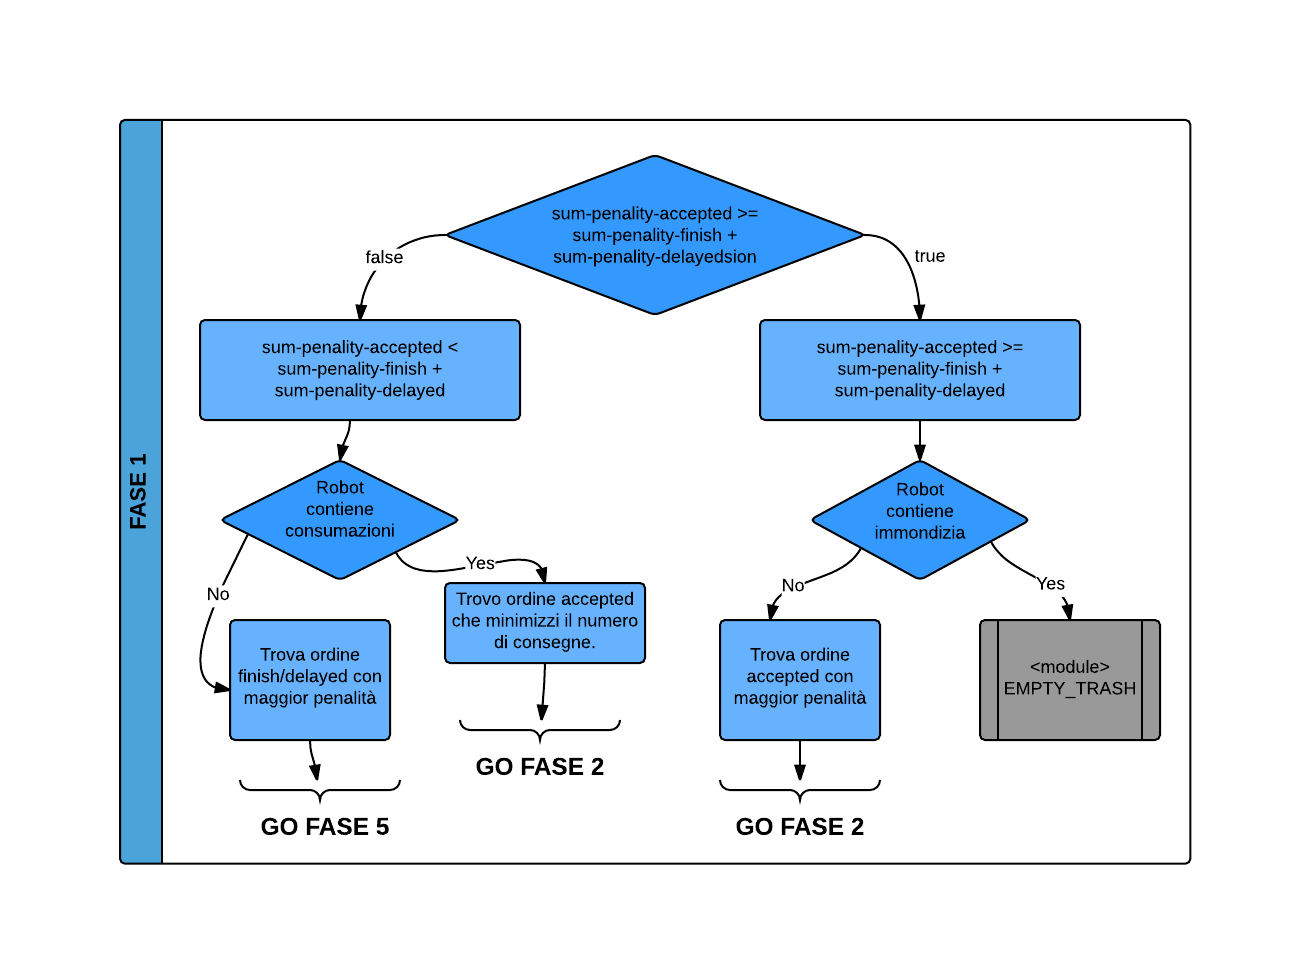
\includegraphics[width=\textwidth]{HARD_fase1}
  \caption{Fase 1 della strategia HARD}
  \label{fig:figure7}
\end{figure}

\begin{equation}
\label{eqn:ordine}
Ordine=\max(x1,x2+x3).
\end{equation}
\[
x1=\sum_{k=1}^n Ordine_\textup{accepted,k}(pen).
\]\[
x2=\sum_{k=1}^n Ordine_\textup{delayed,k}(pen).
\]\[
x3=\sum_{k=1}^n Ordine_\textup{finish,k}(pen).
\]

Dalla formula \eqref{eqn:ordine} si deduce qual'è l'insieme di ordini che a ogni istante di tempo introducono più penalità nel sistema. Una volta individuato questo insieme si cerca al suo interno l'ordine con penalità maggiore. Tale ordine verrà servito.
In alcuni casi il robot prima di servire tale ordine deve compiere delle altre operazioni:
\begin{itemize}
  \item l'ordine da evadere è una finish o delayed ma ho delle consumazioni a bordo, il robot deve consegnare le consumazioni che ha prima di servire l'ordine finish o delayed. Di conseguenza bisogna cercare uno o più ordini accepted. L'idea che sta alla base della ricerca in questo caso è quella di trovare l' ordine o gli ordini che minimizzino il numero di consegne. Se il robot si trova in una situazione di 1drink e 1food preferirà consegnare le consumazioni a un singolo tavolo invece che a due diversi.
  \item l'ordine da evadere è un accepted ma il robot ha sporco a bordo, il sistema forza il robot a recarsi ai cestini.
\end{itemize}

La fase 2 e 3 sono quasi identiche alle precedenti. La fase 2 viene eseguita solo nel caso di ordini accepted, quindi si ricercherà solo il dispenser più vicino al robot.

\begin{figure}[htp]
  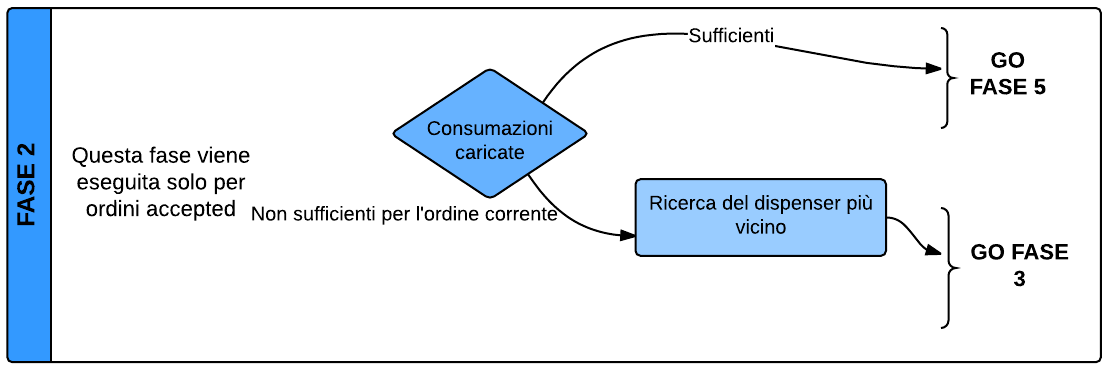
\includegraphics[width=\textwidth]{HARD_fase2}
  \caption{Fase 2 della strategia HARD}
  \label{fig:figure8}
\end{figure}

Nella fase 4, ovvero il caricamento dai dispenser delle consumazioni, abbiamo introdotto la possibilità di caricare le consumazioni per più ordini. Quando il robot arriva a un dispenser carica le consumazioni per l'ordine corrente. Se ha ancora spazio a disposizione e vi sono conumazioni di altri ordini da poter caricare vengono caricate fino al raggiungimento della capacità massima.
La fase 4.5 è molto più semplice delle precedenti. Il fatto di trattare e gestire la pulizia dei tavoli nel modulo EMPTY TRASH ha reso meno complicate alcune fasi.

\begin{figure}[htp]
  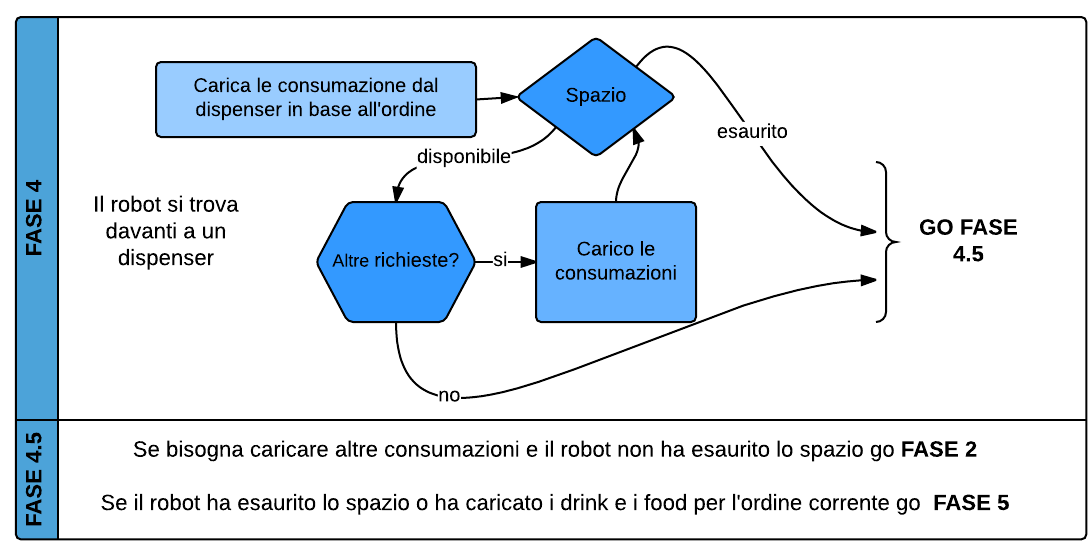
\includegraphics[width=\textwidth]{HARD_fase4_45}
  \caption{Fase 4 e 4.5 della strategia HARD}
  \label{fig:figure9}
\end{figure}

La fase 5 ovvero la ricerca e l'esecuzione del piano per arrivare al tavolo rimane immutata, e non la descriviamo nuovamente.


Nella fase 6 si consegnano le consumazioni al tavolo se era un ordine di accepted o si pulisce il tavolo se era un ordine di finish o delayed.
Nel primo caso potrebbe capitare che l'ordine non risulti completamente evaso, e come nella strategia LOW PENALITY, quest'ordine torna nella lista di ordini da evadere aggiornando le consumazioni da portare in base a quelle già consegnate.
Nel caso sia un ordine di finish oltre a pulire il tavolo l'ordine viene impostato come completato, cosa che non accadeva nelle altre strategie.
Nel caso sia un ordine di delayed l'ordine viene impostato ad accepted e torna nella lista di ordini da evadere. In entrambi i casi il robot ha dello sporco a bordo, ma sarà la fase 1 della strategia che indicherà al robot di andare ai cestini.

\begin{figure}[htp]
  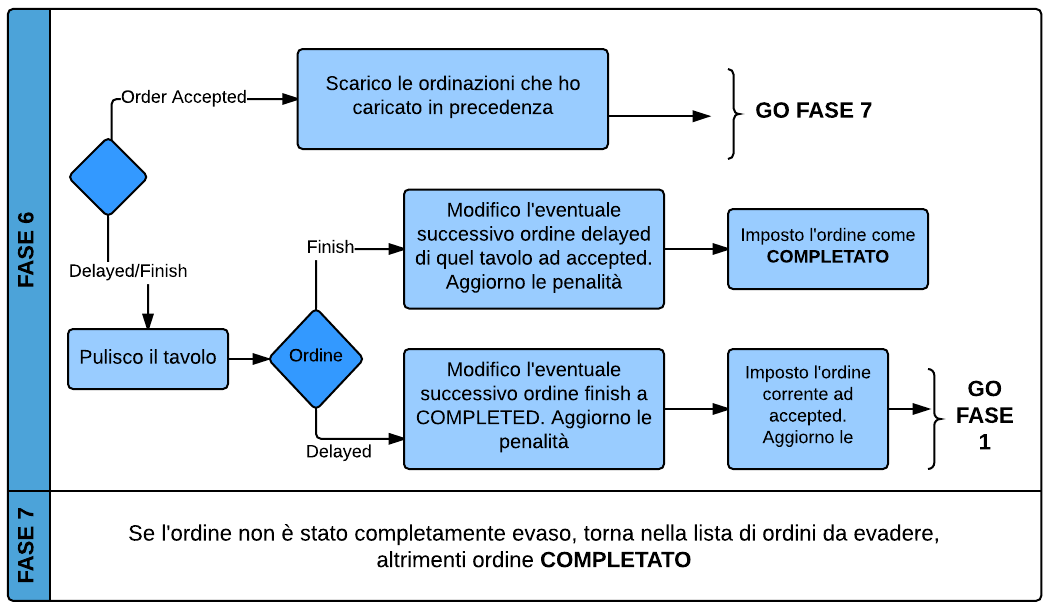
\includegraphics[width=\textwidth]{HARD_fase6-7}
  \caption{Fase 6 e 7 della strategia HARD}
  \label{fig:figure10}
\end{figure}

\subsection{Modulo EMPTY TRASH}
Questo modulo si occupa di liberare dallo sporco il robot. A differenza delle altre strategia, che ogni volta che si puliva un tavolo si cercava anche di liberarsi dello sporco, in questa la pulizia avviene soltanto nei seguenti casi (vedi \ref{fig:figure7}):
\begin{itemize}
  \item l'ordine da evadere è un accepted ma il robot ha sporco a bordo, il sistema forza il robot a recarsi ai cestini.
  \item il robot non ha ordini da completare, prima di fare delle wait prova a liberarsi dello sporco se ne ha.
\end{itemize}

Anche questo modulo è stato suddiviso in 4 fasi:
\begin{itemize}
  \item FASE 0: si individuano quali sono i cestini servibili.
  \item FASE 1: si individua il cestino più vicino (equivalente alla fase 2 delle strategia HARD)
  \item FASE 2: si pianifica e si esegue il piano per arrivare al cestino (equivalente alla fase 3/5 delle strategia HARD)
  \item FASE ND: insieme di azioni da eseguire nel caso A* non trovi una soluzione.
  \item FASE 3: il robot scarica l'immondizia nel cestino
  \item FASE 4: si ritorna alla strategia HARD dove verrà eseguita la FASE 1. Se il robot non ha più sporcizia è pronto per servire ordini accepted altrimente rieseguirà il modulo EMPTY TRASH.
\end{itemize}

Si è dovuto gestire il caso in cui A* fallisca. Una prima soluzione in caso A* fallisca poteva esser quella di aspettare fin quando il basket diventava accessibile, ma risulta essere una soluzione troppo costosa. Il robot potrebbe compiere delle operazioni invece che aspettare. Le azioni che abbiamo individuato sono le seguenti:
\begin{itemize}
  \item la ricerca di un altro cestino se esiste
  \item la ricerca di un altro ordine da servire. Questo significa tornare alla strategia HARD e forzare il robot a evadere un ordine finish o delayed (sono gli unici ordini su cui possiamo operare anche se il robot ha lo sporco).
  \item effettuare delle checkfinish. Se non vi sono ordini finish possiamo cercare se vi sono degli ordini accepted le cui consumazioni sono state consumate e quindi è possibile effettuare un operazione di pulizia del tavolo.
\end{itemize}

\subsection{Checkfinish}
La stategy HARD utilizza anche il comando checkfinish, per controllare se il tavolo ha finito di consumare. Questo comando può esser utilizzato per pulire un tavolo senza aspettare un ordine di finish. Questo non ha un impatto immediato sulle penalità, ma se il robot pulisce un tavolo tramite tale criterio, e successivamente arriva un ordine finish, allora il robot si troverà in uno stato in cui ha già pulito il tavolo e l'ordine non viene preso in cosiderazione. Al contrario dovrà prendere in consegna l'ordine e accumulare delle penalitò fin quando non sarà evaso.
Questa modalità viene attivata quando il robot non ha ordini da evadere. L'idea è quella di portarsi avanti ipotizzando ordini successivi per i tavoli attualmente sporchi, e quindi decidendo di pulirli nel caso la risposta al comando checkfinish sia positiva. Quindi quando il robot non ha ordini pendenti, si reca a ogni tavolo sporco ed effettua una checkfinish. Se la risposta è positiva carica lo sporco. Se non sono arrivati altri ordini ripete tale operazione per il successivo tavolo sporco. Se non ci sono più tavoli sporchi o se è arrivato un ordine si reca ai cestini.


\subsection{Vantaggi e Svantaggi}
Anche in questa stategia è possibile come nelle precedenti una situazione di stallo(\ref{fig:figure6}).
Ipotizziamo per questa strategia due grossi vantaggi. Il primo è quello che riesce a servire più ordini in contemporanea, quindi in particolari situazione è in grado di recarsi una sola volta ai vari dispenser e riuscire a completare più ordini provenienti da tavoli diversi. L'altro vantaggio è dato dalla checkfinish, che permette al robot di trovarsi in uno stato con tutti i tavoli puliti e quindi pronto a servire i successivi ordini.
Questa strategia potrebbe dover tornare a un tavolo più volte rispetto alle precedenti, e con mappe molto grosse questo potrebbe risultare un problema. Supponiamo di avere 2 ordini uno proveniente dal tavolo T1 con la richiesta di 2 food e 2 drink, e uno dal tavolo T2 con 2 food e 1 drink. Le altre strategia che servono un ordine per volta, caricherebbero 2 food e 2 drink completando l'ordine T1. Mentre questa strategia caricherebbe 4 food e ne consegnerebbe 2 a T1 e 2 a T2. In questo modo deve tornare una seconda volta al tavolo T1 per la completare la richiesta con 2 drink.
Un altro svantaggio potrebbe verificarsi durante le operazioni di checkfinish. Supponiamo che il robot non abbia ordini da evadere e inizia le operazioni di checkfinish e inizia a pulire i tavoli. Se arriva un ordine accepted il robot a differenze delle altre strategie non potrà iniziare subito le operazioni di evasione, ma dovrà prima completare l'ordine fittizio di checkfinish che ha preso in carico e poi recarsi ai cestini per svuotare lo sporco, accumulando penalità.

\section{Risultati}
Le quattro strategie sono state create in maniera incrementale, aggiungendo regole e modificandone alcune al fine di migliorare le prestazioni delle strategie e minimizzare la penalità accumulata. Al fine di confermare queste ipotesi abbiamo creato un gruppo di history per trarre conclusioni e fare assunzioni basate su dati certi, le \emph{Final Results History}.

Un altro gruppo di history, creato per testare le strategie stesse, affinché si compostassero come previsto, è stato creato durante lo sviluppo. Oltre a testare le nostre strategie possono già fornire delle indicazioni sulla bontà della strategia.

\subsection{Testing Histories}
Le testing history sono cinque: default, complicata, dave, wait, andrea.

\subsubsection{History \emph{default}}
E' la history inclusa nel progetto.

\begin{table}[h]
\begin{tabular}{|l|l|l|l|l|l|}
\hline
                 & BASE & PRO   & LOW\_PENALTY  & PENDIST & HARD \\ \hline
Penalty          & 1452 & 1452  & 1452          & 1452    & 676  \\ \hline
Reused planes    & 1    & 1     & 1             & 1       & 0    \\ \hline
Orders performed & 4    & 4     & 0             & 0       & 1    \\ \hline
Total orders     & 4    & 4     & 4             & 4       & 2    \\ \hline
\end{tabular}
\end{table}

Le prime quattro strategie hanno il medesimo comportamento,in quanto l'ordine con cui evadere gli ordini è lo stesso. La strategy HARD pur servendo gli ordini nello stesso ordine delle altre, ha bisogno di più step quando si reca al food-dispenser in quanto carica le consumazioni per più ordini. Questo fa si che il tavolo T4 venga servito in ritardo rispetto alle altre strategie e non permette al sistema di prendere in carico i successivi due ordini di quel tavolo che avvengono prima che il robot abbia finito di consegnare le consumazioni richieste.

\subsubsection{History \emph{complicata}}

\begin{table}[h]
\begin{tabular}{|l|l|l|l|l|l|}
\hline
                 & BASE & PRO   & LOW\_PENALTY  & PENDIST & HARD  \\ \hline
Penalty          & NaN  & 4080  & 5367          & 4348    & 4736   \\ \hline
Reused planes    & NaN  & 3     & 4             & 4       & 1      \\ \hline
Orders performed & NaN  & 8     & 9             & 8       & 6+(2)  \\ \hline
Total orders     & NaN  & 9     & 9             & 9       & 9      \\ \hline
\end{tabular}
\end{table}

La strategy FIFO BASE non ripianificando non termina in quanto il robot trova sul suo percorso una persona. La strategy HARD sembra servire meno tavoli rispetto le altre strategie. In realtà la strategy HARD effettua delle checkfinish pulendo i tavoli, quindi gli ordini successivi di finish non vengono presi in considerazione in quanto i tavoli sono già puliti. Tra parentesi sono indicati gli ordini di finish non ricevuti dal sistema perchè in precedenza erano già state effettuate delle checkfinish. La checkfinish viene attivata quando il robot non ha nessun ordine da servire. Se un ordine arriva mentre si stanno svolgendo le operazioni di checkfinish, prima di poterlo servire e quindi azzerare le penalità dovute a tale ordine, si dovranno concludere prima le operazioni di checkfinish. Nell'esempio l'operazione di checkfinish porta alla pulizia di tutti i tavoli sporchi.
La differenza tra FIFO PRO e LOW PENALITY ci porta a capire che la scelta di servire prima i tavoli con più penalità non è sempre la migliore, in quanto bisogna tenere in considerazione anche le distanza che il robot deve coprire per servire tale ordine. Ciò nonostante anche la strategy PENDIST si comporta pegggio di FIFO PRO. Analizzando il numero di step imiegati per servire ciascun ordine da entrambe le strategie si nota come per servire il tavolo T3 con ordinazine food:3 e drink:2, FIFO PRO impiega 21 step mentre PENDIST ben 43. Questo perchè il robot troverà nel suo percorso una persona e dovrà ricalcolare e eseguire un piano diverso e più lungo per arrivare a destinazione.

\subsubsection{History \emph{dave}}

\begin{table}[h]
\begin{tabular}{|l|l|l|l|l|l|}
\hline
                 & BASE & PRO   & LOW\_PENALTY  & PENDIST & HARD    \\ \hline
Penalty          & NaN  & 3841  & 3841          & 3841    & 6092   \\ \hline
Reused planes    & NaN  & 1     & 1             & 1       & 3      \\ \hline
Orders performed & NaN  & 7     & 7             & 7       & 6+(5)  \\ \hline
Total orders     & NaN  & 11    & 11            & 11      & 11     \\ \hline
\end{tabular}
\end{table}

La strategy FIFO BASE non ripianificando non termina in quanto il robot trova sul suo percorso una persona.
La strategy HARD è l'unica strategia che riesce a servire tutti gli ordini. Con questo esempio notiamo come affidarci solo alle penalità per confrontare le varie strategie non è una buona idea. Si potrebbe calcolare la penalità media di ogni ordine. Ma anche in questo caso il risultato non riuscirebbe a fornirci un'indicazione molto precisa. Nell'esempio per le prime 4 strategia si avrebbe una penalità media per ordine di 549, mentre per la HARD di 553. I primi 4 ordini di questa history vengono serviti da tutte le strategie, ma mentre le prime 4 impiegano 136 step per servirli, la HARD solo 92. In seguito le altre strategie accumuleranno solo le penalità relative a 3 ordini, mentre la HARD le penalità relative a 7 ordini.
Un'altro importante commento che possiamo effettuare osservando i risultati è come history con idee molto diverse tra di loro per servire gli ordini (una basata sull'ordine di arrivo, una basata sulle penalità e l'altra sulle penalità e distanze) abbiano un comportamento simile.

\subsubsection{History \emph{wait}}

\begin{table}[h]
\begin{tabular}{|l|l|l|l|l|l|}
\hline
                 & BASE & PRO   & LOW\_PENALTY  & PENDIST & HARD   \\ \hline
Penalty          & 3117 & 3425  & 2825          & 2875    & 2596   \\ \hline
Reused planes    & 2    & 2     & 2             & 1       & 0      \\ \hline
Orders performed & 5    & 5     & 5             & 5       & 5      \\ \hline
Total orders     & 5    & 5     & 5             & 5       & 5      \\ \hline
\end{tabular}
\end{table}

La FIFO BASE si comporta meglio della FIFO PRO in quanto ricadiamo nel caso in cui aspettare che la persona si muova invece di ripianificare ci permette di risparmiare.

\subsection{Final Results Histories}

Per ottenere i risultati finali sulle strategie sono state create tre mappe e sei history diverse per ogni mappa. Le mappe sono di tre dimensioni diverse: \emph{10x10} blocchi, \emph{20x20} e \emph{30x30}; mentre le cinque history sono state etichettate come: \emph{hdefault}, \emph{hsimple}, \emph{hhard}, \emph{hperson1}, \emph{hperson2} e \emph{hcheckf}. Ogni history rappresenta uno scenario particolare.

La history default presenta le seguenti caratteristiche:
\begin{itemize}
  \item poche persone che si muovono.
  \item presenza sia di ordini con molte richieste, sia di ordini con poche richieste.
\end{itemize}
La history hsimple presenta le seguenti caratteristiche:
\begin{itemize}
    \item non vi sono persone che si muovono.
    \item presenza solo di ordini con poche richieste.
  \end{itemize}
La history hhard presenta le seguenti caratteristiche:
\begin{itemize}
    \item non vi sono persone che si muovono.
    \item presenza solo di ordini con tante richieste.
  \end{itemize}
La history hperson1 presenta le seguenti caratteristiche:
\begin{itemize}
    \item molte persone che si muovono di continuo. Ogni persona si sposta da un punto A a B e viceversa.
    \item presenza sia di ordini con molte richieste, sia di ordini con poche richieste.
  \end{itemize}
La history hperson2 presenta le seguenti caratteristiche:\begin{itemize}
    \item molte persone che si muovono di continuo. Ogni persona si sposta da un punto A a B e viceversa. A differenza della hperson1 che ad ogni step una persona si muove, nella hperson2 lo spostamento avviene ogni x step. Con x che varia da 1 a 4.
    \item presenza sia di ordini con molte richieste, sia di ordini con poche richieste.
  \end{itemize}
La history hcheckf presenta le seguenti caratteristiche:
\begin{itemize}
    \item non vi sono persone che si muovono.
    \item presenza sia di ordini con molte richieste, sia di ordini con poche richieste.
    \item history create in modo tale da utilizzare l'azione di checkfinish da parte della strategia HARD.
\end{itemize}


\subsubsection{Risultati sulla mappa 10x10: hdefault}
\begin{table}[h]
\begin{tabular}{|c|c|c|c|l|l|}
\hline
\multicolumn{1}{|l|}{} & BASE  & PRO   & LOW\_PENALTY  & PENDIST & HARD \\ \hline
Penalty                & 5837  & 5616  & 4192          & 3810    & 4170 \\ \hline
Reused Planes          & 2     & 4     & 5             & 2       & 0    \\ \hline
Order performed        & 7     & 7     & 6             & 7       & 6    \\ \hline
Total orders           & 10    & 10    & 10            & 10      & 10   \\ \hline
\end{tabular}
\end{table}

Dalla tabella notiamo che la strategy PENDIST è quella che minimizza la nostra penalità su quest'history.
Un'altro dato importante è il numero di ordini presi in carico dal sistema. Questo numero può variare a seconda della strategia in esecuzione in quanto ordini inseriti nella history non sono consistenti con tale esecuzione e non vengono presi in carico dal sistema. Per questo motivo un metro di giudizio non è stato il valore della penalty, ma la penalty media per ogni ordine.

Come precedentemente spiegato nel capitolo \ref{sec:modulo_astar} i piani principali vengono salvati. I risultati sulla riga Reused Plane codificano l'informazione riguardante questa idea. Ricordiamo che il fatto di riutilizzare un piano non ci dà dei guadagni dal punto di vista della penalità. Notiamo che la strategy HARD non riutilizza nessun piano (prima di commentare questo risultato valuteremo anche i dati provenienti dalle altre history per vedere se è una casualità o se è un risultato determinato da come la strategy HARD serve gli ordini)

Dall'esecuzione della FIFO BASE e FIFO PRO su questa history si ha un primo confronto tra l'idea di aspettare nel caso in cui vi sia una persona sul percorso del robot, e quella della FIFO PRO di ripianificare. Notiamo che anche se il robot deve ripianificare e allungare i tempi di consegna per via dell'esecuzione di un altro percorso, la penalità risulta migliore rispetto al fatto di aspettare anche se per pochi step (3 nella nostra esecuzione). La FIFO BASE completa i suoi ordini in 171 step mentre la FIFO PRO in 176.


\subsubsection{Risultati sulla mappa 10x10: hsimple}
\begin{table}[h]
\begin{tabular}{|c|c|c|c|l|l|}
\hline
\multicolumn{1}{|l|}{} & BASE & PRO   & LOW\_PENALTY & PENDIST & HARD \\ \hline
Penalty                & 1527 & 1527  & 1661         & 1543    & 1334 \\ \hline
Reused Planes          & 5    & 5     & 4            & 2       & 1    \\ \hline
Order performed        & 11   & 11    & 11           & 11      & 11   \\ \hline
Total orders           & 12   & 12    & 12           & 12      & 12   \\ \hline
\end{tabular}
\end{table}

La strategy HARD riuscendo a serivire più ordini insieme risulta esser la migliore.

\subsubsection{Risultati sulla mappa 10x10: hhard}
\begin{table}[h]
\begin{tabular}{|c|c|c|c|l|l|}
\hline
\multicolumn{1}{|l|}{} & BASE  & PRO    & LOW\_PENALTY & PENDIST & HARD  \\ \hline
Penalty                & 14966 & 14966  & 14651        & 13888   & 10543 \\ \hline
Reused Planes          & 14    & 14     & 14           & 14      & 3     \\ \hline
Order performed        & 9     & 9      & 9            & 9       & 9     \\ \hline
Total orders           & 12    & 12     & 12           & 12      & 12    \\ \hline
\end{tabular}
\end{table}

La strategy HARD avendo per ogni ordine un numero molto alto di richieste costringe il robot a effettuare più volte delle consegne allo stesso tavolo. Questo giustiifica sia i valori di penalità molto alti sia il numero di piani riusati per arrivare a destinazione.

\subsubsection{Risultati sulla mappa 10x10: hperson1}
\begin{table}[h]
\begin{tabular}{|c|c|c|c|l|l|}
\hline
\multicolumn{1}{|l|}{} & BASE & PRO   & LOW\_PENALTY & PENDIST & HARD    \\ \hline
Penalty                & NaN  & 11711 & 6943         & 6943    & 6741    \\ \hline
Reused Planes          & NaN  & 8     & 7            & 7       & 0       \\ \hline
Order performed        & NaN  & 11    & 11           & 11      & 11      \\ \hline
Total orders           & NaN  & 12    & 12           & 12      & 12      \\ \hline
\end{tabular}
\end{table}

La strategy FIFO WAIT non termina in quanto si arriva in una situazione di deadlock. LOW PENALTY e PENDIST servono gli ordini allo stesso modo e quindi hanno il medesimo comportamento. La strategy HARD effettua delle checkfinish.

\subsubsection{Risultati sulla mappa 10x10: hperson2}
\begin{table}[h]
\begin{tabular}{|c|c|c|c|l|l|}
\hline
\multicolumn{1}{|l|}{} & BASE & PRO     & LOW\_PENALTY & PENDIST & HARD     \\ \hline
Penalty                & NaN  & 7594    & 8235         & 8235    & 6755     \\ \hline
Reused Planes          & NaN  & 7       & 8            & 8       & 3        \\ \hline
Order performed        & NaN  & 9       & 11           & 11      & 7        \\ \hline
Total orders           & NaN  & 12      & 12           & 12      & 12       \\ \hline
\end{tabular}
\end{table}

In questo caso le varie strategie riescono a servire un numero di ordini sensibilmente diverso, dai soli 7 della HARD ai ben 11 di PENDSIT e LOW PENALTY.

\subsubsection{Risultati sulla mappa 10x10: hcheckf}
\begin{table}[h]
\begin{tabular}{|c|c|c|c|l|l|}
\hline
\multicolumn{1}{|l|}{} & BASE & PRO     & LOW\_PENALTY & PENDIST & HARD     \\ \hline
Penalty                & 4964 & 4964    & 3840         & 3796    & 3336     \\ \hline
Reused Planes          & 8    & 8       & 5            & 8       & 5        \\ \hline
Order performed        & 12   & 12      & 12           & 12      & 12       \\ \hline
Total orders           & 12   & 12      & 12           & 12      & 12       \\ \hline
\end{tabular}
\end{table}

La strategy HARD su questa mappa almeno teoricamente dovrebbe avere un grosso vantaggio dato dal fatto che se il robot è in uno stato di riposo in quanto ha già servito tutti gli ordini pendenti, invece di rimanere in uno stato non operativo controlla se ci sono tavoli che possono esser puliti, tramite il comando di checkfinish. In questo modo si trova in uno stato migliore rispetto le altre strategie dovessero arrivare nuovi ordini.

\subsubsection{Grafici Mappa 10x10}
\begin{figure}[htp]
  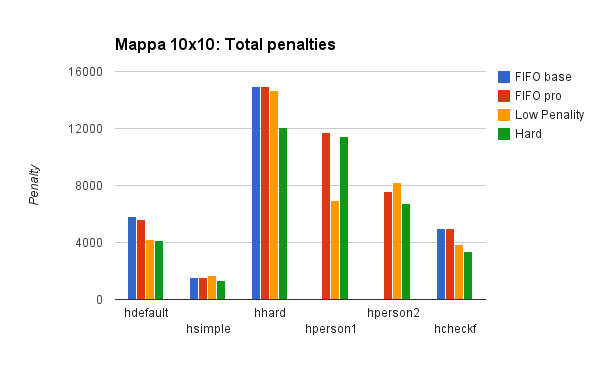
\includegraphics[width=\textwidth]{10x10_penalties}
  \caption{Grafico Penalità mappe 10x10}
  \label{fig:10x10figure11}
\end{figure}

\begin{figure}[htp]
  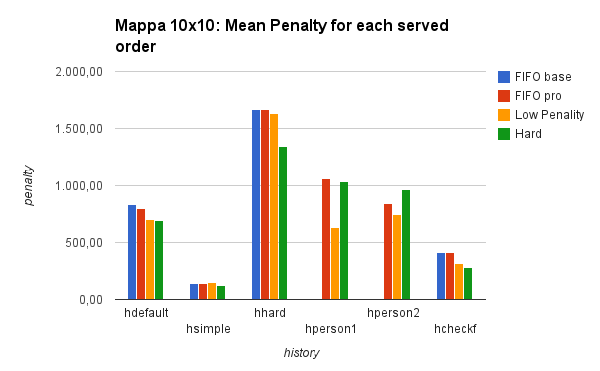
\includegraphics[width=\textwidth]{10x10_mean_pen}
  \caption{Grafico penalità media per ordine}
  \label{fig:10x10figure12}
\end{figure}

\subsubsection{Risultati sulla mappa 20x20: hdefault}
\begin{table}[h]
\begin{tabular}{|c|c|c|c|l|l|}
\hline
\multicolumn{1}{|l|}{} & BASE   & PRO   & LOW\_PENALTY & PENDIST & HARD \\ \hline
Penalty                & 2172   & 2172  & 2257         & 2257    & 2208 \\ \hline
Reused Planes          & 0      & 0     & 0            & 0       & 0    \\ \hline
Order performed        & 6      & 6     & 6            & 6       & 6    \\ \hline
Total orders           & 6      & 6     & 6            & 6       & 6    \\ \hline
\end{tabular}
\end{table}

Il discorso precedentemente fatto per le mappe 10x10 vale anche nel caso in cui ci troviamo a lavorare con mappe 20x20.Le variabili considerate  in questo caso sono le stesse descritte precedentemente di modo da avere risultati consistenti ed equiparabili.
Dall'esecuzione delle strategie su questa history si nota che si comportano più o meno tutte allo stesso modo con uno scarto minimo. Vista la semplicità della history sottoposta alle strategie, FIFO\_BASE e FIFO\_PROsi comportano un pochino meglio delle più complesse strategie LOW\_PENALTY, HARD  e PENDIST  anche se come abbiamo già detto la differenza è minima.

\subsubsection{Risultati sulla mappa 20x20: hsimple}
\begin{table}[h]
\begin{tabular}{|c|c|c|c|l|l|}
\hline
\multicolumn{1}{|l|}{} & BASE  & PRO    & LOW\_PENALTY & PENDIST  & HARD \\ \hline
Penalty                & 4694  & 4694   & 4439         & 4016     & 3966 \\ \hline
Reused Planes          & 1     & 1      & 1            & 1        & 0    \\ \hline
Order performed        & 12    & 12     & 12           & 12       & 12   \\ \hline
Total orders           & 13    & 13     & 13           & 13       & 13   \\ \hline
\end{tabular}
\end{table}

Dall'esecuzione delle strategie su questa history notiamo subito che nessuna riesce ad eseguire tutti gli ordini presenti nella history. FIFO\_BASE e FIFO\_PRO hanno un esecuzione identica e quindi penalità uguale, mentre LOW\_PENALITY si comporta un pochino meglio servendo lo stesso numero di ordini ma con 255 penalità in meno. PENDIST riesce a fare decisamente meglio di LOW\_PENALTY, risparmiando ben 423 penalità, a fronte dello stesso numero di ordini serviti. HARD pur non riutilizzando nessun piano è la strategia che si comporta meglio di tutte risparmiando ulteriormente 473 penalità in confronto a LOW\_PENALTY e 50 in confronto a PENDIST.

\subsubsection{Risultati sulla mappa 20x20: hhard}
\begin{table}[h]
\begin{tabular}{|c|c|c|c|l|l|}
\hline
\multicolumn{1}{|l|}{} & BASE   & PRO        & LOW\_PENALTY & PENDIST & HARD \\ \hline
Penalty                & 38360  & 38360      & 26596        & 26925   & 25422 \\ \hline
Reused Planes          & 10     & 10         & 6            & 8       & 2    \\ \hline
Order performed        & 15     & 15         & 13           & 13      & 12  \\ \hline
Total orders           & 15     & 15         & 15           & 15      & 15  \\ \hline
\end{tabular}
\end{table}

Dall'esecuzione della strategia notiamo subito 2 cose: l'esecuzione di FIFO\_BASE e FIFO\_PRO è identica, questo perchè come già detto l'agente non incontra persone ad ostacolarlo lungo i suoi percorsi; la seconda cosa è che LOW\_PENALTY, PENDIST e HARD non servono tutti gli ordini della history e quindi hanno tempi di esecuzione decisamente minori delle strategie FIFO\_BASE e FIFO\_PRO. Un altro fatto che balza all'occhio è il forte riutilizzo dei piani (ben 10) da parte di FIFO\_BASE e FIFO\_PRO e ben 8 da parte di PENDIST; in misura minore anche LOW\_PENALTY fa uso di questa feature mentre HARD la usa decisamente poco in questa history.

\subsubsection{Risultati sulla mappa 20x20: hperson1}
\begin{table}[h]
\begin{tabular}{|c|c|c|c|l|l|}
\hline
\multicolumn{1}{|l|}{} & BASE & PRO        & LOW\_PENALTY & PENDIST & HARD   \\ \hline
Penalty                & NaN  & 20873      & 18166        & 15737   & 13607  \\ \hline
Reused Planes          & NaN  & 4          & 3            & 3       & 2      \\ \hline
Order performed        & NaN  & 15         & 15           & 15      & 13     \\ \hline
Total orders           & NaN  & 15         & 15           & 15      & 15     \\ \hline
\end{tabular}
\end{table}

Dall'esecuzione della strategia notiamo subito l'assenza di valore per la strategia FIFO\_BASE; questo è completamente lecito perchè durante l'esecuzione l'agente entra in un attesa infinita aspettando che una persona si sposti, ma dato che la persona vuole andare proprio nella cella occupata dall'agente si crea un deadlock e l'esecuzione non può essere portata a termine. Altro fatto di rilievo è dato dalla strategia HARD che evade 13 ordini anzichè 15 e di conseguenza il suo risultato va preso con le pinze. LOW\_PENALTY e PENDIST evadono tutti gli ordini con PENDIST che risulta decisamente migliore della prima, riuscendo a risparmiare circa 3000 penalità.

\subsubsection{Risultati sulla mappa 20x20: hperson2}
\begin{table}[h]
\begin{tabular}{|c|c|c|c|l|l|}
\hline
\multicolumn{1}{|l|}{} & BASE & PRO     & LOW\_PENALTY & PENDIST & HARD   \\ \hline
Penalty                & NaN  & 21049   & 17665        & 12830   & 13761  \\ \hline
Reused Planes          & NaN  & 7       & 6            & 6       & 2      \\ \hline
Order performed        & NaN  & 13      & 15           & 13      & 15     \\ \hline
Total orders           & NaN  & 15      & 15           & 15      & 15     \\ \hline
\end{tabular}
\end{table}

Anche in questa mappa FIFO\_BASE non termina la sua esecuzione, per la stessa ragione esposta per la mappa hperson1. PENDIST e FIFO\_PRO evadono 13 ordini su 15; FIFO\_PRO risulta la peggiore di tutte pur eseguendo 2 ordini in meno, mentre PENDIST risulta la migliore di tutte, anche se il suo risultato va comunque preso con le pinze. LOW\_PENALTY e HARD evadono tutti gli ordini con la strategia HARD che riesce a risparmiare circa 3000 penalità nei confronti di LOW\_PENALTY.


\subsubsection{Risultati sulla mappa 20x20: hcheckf}
\begin{table}[h]
\begin{tabular}{|c|c|c|c|l|l|}
\hline
\multicolumn{1}{|l|}{} & BASE  & PRO     & LOW\_PENALTY & PENDIST & HARD   \\ \hline
Penalty                & 16664 & 13961   & 13961        & 14145   & 12780  \\ \hline
Reused Planes          & 10    & 6       & 6            & 5       & 4      \\ \hline
Order performed        & 15    & 15      & 15           & 15      & 15     \\ \hline
Total orders           & 15    & 15      & 15           & 15      & 15     \\ \hline
\end{tabular}
\end{table}

Per quanto riguarda questa strategia tutte le strategie evadono tutti gli ordini. FIFO\_BASE risulta la peggiore di tutte dato che l'agente è costretto a perdere del tempo prezioso in attesa che le persone gli lascino campo libero per poter proseguire a servire i tavoli.PENDIST risulta migliore della strategia di base, ma leggermente peggiore delle strategie FIFO\_PRO e LOW\_PENALTY le quali risultano in questo caso identiche; questo è dovuto al semplice fatto che prendendo in carico gli ordini allo stesso modo i passi dell'agente risultano i medesimi per entrambe le strategie e dato che la gestione delle interferenza da parte delle persone è la medesima, la penalità accumulata è uguale. HARD si dimostra la migliore delle cinque riuscendo a portare a termine tutta la history con penalità più bassa

\subsubsection{Grafici Mappa 20x20}
\begin{figure}[htp]
  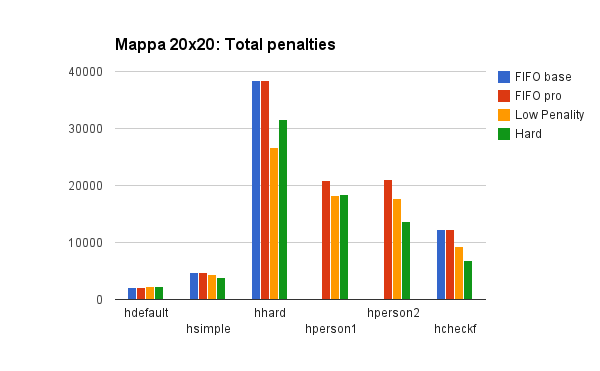
\includegraphics[width=\textwidth]{20x20_penalties}
  \caption{Grafico Penalità mappe 10x10}
  \label{fig:20x20pen}
\end{figure}

\begin{figure}[htp]
  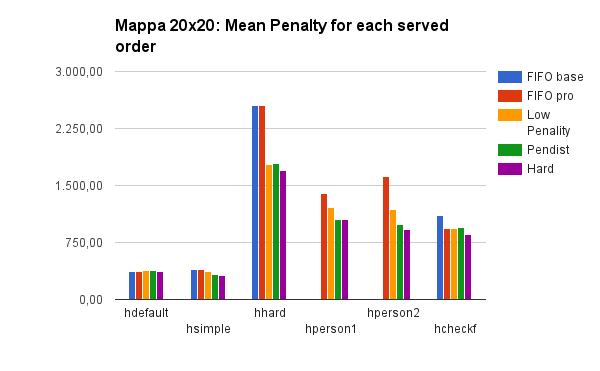
\includegraphics[width=\textwidth]{20x20_mean_pen}
  \caption{Grafico penalità media per ordine}
  \label{fig:20x20meanpen}
\end{figure}


\subsubsection{Risultati sulla mappa 30x30: hdefault}
\begin{table}[h]
\begin{tabular}{|c|c|c|c|l|l|}
\hline
\multicolumn{1}{|l|}{} & BASE   & PRO   & LOW\_PENALTY & PENDIST & HARD \\ \hline
Penalty                & 10763  & 10763 & 8737         & 8229    & 8469 \\ \hline
Reused Planes          & 1      & 1     & 1            & 2       & 0    \\ \hline
Order performed        & 7      & 7     & 7            & 7       & 7    \\ \hline
Total orders           & 9      & 9     & 9            & 9       & 9    \\ \hline
\end{tabular}
\end{table}

Anche in questo caso vale quanto detto per le mappe 10x10 e 20x20. I paramentri di valutazione sono invariati anche per i test sulle mappe 30x30, sempre per poter avere tutti i risultati consistenti ed equiparabili.
Dall'esecuzione della history notiamo che tutte le strategie eseguono 7 ordini su 9 e che l'esecuzione della FIFO\_BASE e FIFO\_PRO è identica. LOW\_PENALTY e HARD si comportano decisamente meglio delle semplici FIFO\_BASE e FIFO\_PRO, ma per questa history la migliore risulta PENDIST risparmiando ulteriori 267 penalità nei confronti della HARD.

\subsubsection{Risultati sulla mappa 30x30: hsimple}
\begin{table}[h]
\begin{tabular}{|c|c|c|c|l|l|}
\hline
\multicolumn{1}{|l|}{} & BASE  & PRO    & LOW\_PENALTY & PENDIST  & HARD \\ \hline
Penalty                & 13352 & 13352  & 13041        & 14064    & 14052\\ \hline
Reused Planes          & 0     & 0      & 1            & 1        & 0    \\ \hline
Order performed        & 12    & 12     & 13           & 13       & 14   \\ \hline
Total orders           & 20    & 20     & 20           & 20       & 20   \\ \hline
\end{tabular}
\end{table}

Per quanto riguarda l'esecuzione della history hsimple, abbiamo parecchi punti da chiarire. Prima di tutto FIFO\_BASE e FIFO\_PRO sembrano comportarsi disceramente bene per questa history, ma il loro ``buon risultato'' va preso con le pinze dato che, a differenza delle altre strategie, eseguono un numero minore di ordini. Stesso discorso vale per PENDIST ma sopratutto per LOW\_PENALTY che sembrerebbe essere la migliore; pur eseguendo un ordine in più di FIFO\_BASE e FIFO\_PRO ne esegue comunque 1 in meno di HARD. HARD, pur avendo un tempo di esecuzione relativamente alto rapportato con le altre strategie, è quella che è in grado di evadere il maggior numero di ordini in questa history.

\subsubsection{Risultati sulla mappa 30x30: hhard}
\begin{table}[h]
\begin{tabular}{|c|c|c|c|l|l|}
\hline
\multicolumn{1}{|l|}{} & BASE   & PRO        & LOW\_PENALTY & PENDIST & HARD \\ \hline
Penalty                & 49344  & 49344      & 53459        & 51219   & 69313 \\ \hline
Reused Planes          & 5      & 5          & 6            & 3       & 7    \\ \hline
Order performed        & 12     & 12         & 12           & 12      & 12  \\ \hline
Total orders           & 20     & 20         & 20           & 20      & 20  \\ \hline
\end{tabular}
\end{table}

Dall'esecuzione della history notiamo subito che tutte le strategie evadono lo stesso numero di ordini. In questo caso possiamo dire effettivamente che FIFO\_BASE e FIFO\_PRO si comportano meglio delle altre strategie più complesse, riuscendo a risparmiare addirittura 1875 penalità da PENDIST che risulta essere la seconda migliore. HARD in questo caso è quella che si comporta peggio di tutti accumulando circa 20000 penalità in più da FIFO\_BASE e FIFO\_PRO.

\subsubsection{Risultati sulla mappa 30x30: hperson1}
\begin{table}[h]
\begin{tabular}{|c|c|c|c|l|l|}
\hline
\multicolumn{1}{|l|}{} & BASE & PRO        & LOW\_PENALTY & PENDIST & HARD   \\ \hline
Penalty                & NaN  & 28816      & 27850        & 24781   & 33327  \\ \hline
Reused Planes          & NaN  & 1          & 1            & 2       & 2      \\ \hline
Order performed        & NaN  & 12         & 12           & 12      & 12     \\ \hline
Total orders           & NaN  & 20         & 20           & 20      & 20     \\ \hline
\end{tabular}
\end{table}

L'esecuzione di FIFO\_BASE si comporta esattamente come nel dominio precedente (mappe 20x20), lasciando l'agente bloccato in deadlock nell'attesa che la persona si sposti. Il numero di ordini serviti dalle altre strategie è lo stesso e anche in questo caso HARD si comporta peggio delle altre accumulando circa 11000 penalità in più della migliora, che in questo caso è PENDIST. FIFO\_PRO e LOW\_PENALTY risultano migliori di HARD ma hanno uno scarto di circa 3500 penalità da PENDIST.

\subsubsection{Risultati sulla mappa 30x30: hperson2}
\begin{table}[h]
\begin{tabular}{|c|c|c|c|l|l|}
\hline
\multicolumn{1}{|l|}{} & BASE & PRO     & LOW\_PENALTY & PENDIST & HARD   \\ \hline
Penalty                & NaN  & 27495   & 29675        & 25809   & 34061  \\ \hline
Reused Planes          & NaN  & 4       & 0            & 4       & 3      \\ \hline
Order performed        & NaN  & 12      & 12           & 12      & 12     \\ \hline
Total orders           & NaN  & 20      & 20           & 20      & 20     \\ \hline
\end{tabular}
\end{table}

Anche in questa mappa FIFO\_BASE non termina la sua esecuzione, per la stessa ragione esposta per la mappa hperson1. Anche i risultati ottenuti dalle altre strategie sono molto simili a quelli ottenuti con hperson1. HARD è rimasta ancora la peggiore, FIFO\_PRO e LOW\_PENALTY sono decisamenti migliore, ma ancora una volta la migliore risulta PENDIST.

\subsubsection{Risultati sulla mappa 30x30: hcheckf}
\begin{table}[h]
\begin{tabular}{|c|c|c|c|l|l|}
\hline
\multicolumn{1}{|l|}{} & BASE  & PRO     & LOW\_PENALTY & PENDIST & HARD   \\ \hline
Penalty                & 26142 & 26142   & 20737        & 17602   & 10387  \\ \hline
Reused Planes          & 7     & 7       & 6            & 6       & 10     \\ \hline
Order performed        & 20    & 20      & 20           & 20      & 21     \\ \hline
Total orders           & 21    & 21      & 21           & 21      & 21     \\ \hline
\end{tabular}
\end{table}

Dall'esecuzione della history notiamo subito che l'unica strategia che è in grado di evadere la history per intero e la HARD; oltretutto risulta anche essere la strategia più veloce con una penalità accumulata veramente bassa (10387) e uno scarto di circa 7000 penalità dalla seconda migliore che è PENDIST. LOW\_PENALTY si comporta discretamente, ma accumula comunque un numero di penalità superiore a PENDIST e HARD. Le peggiori risultano essere FIFO\_BASE e FIFO\_PRO.

\subsubsection{Grafici Mappa 30x30}
\begin{figure}[htp]
  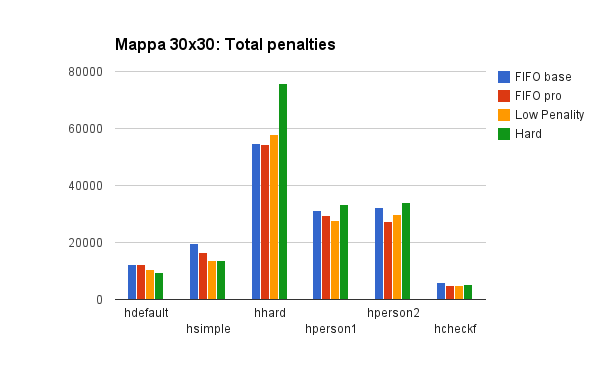
\includegraphics[width=\textwidth]{30x30_penalties}
  \caption{Grafico Penalità mappe 10x10}
  \label{fig:figure11}
\end{figure}

\begin{figure}[htp]
  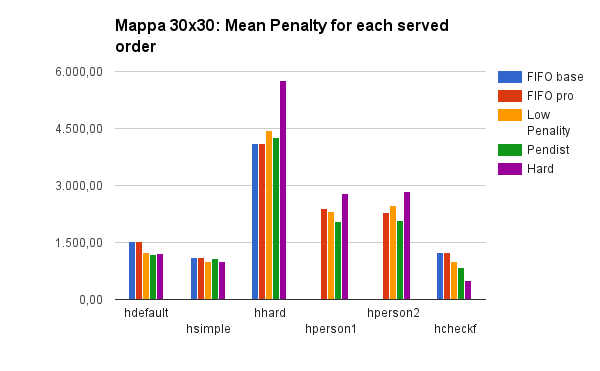
\includegraphics[width=\textwidth]{30x30_mean_pen}
  \caption{Grafico penalità media per ordine}
  \label{fig:figure12}
\end{figure}


\section{Conclusioni}
